\section{Cryogenic ion trap}

An electric field exerts a force on a charged particle, such as an atomic or molecular ion. Earnshaw's \cite{earnshaw_nature_1848} theorem states that it is impossible to maintain stable confinement (i.e., trapping) of charged particles by static electric fields. However, it is possible to trap ions in stable confinement using time-varying (rf - radiofrequency) electric fields. Since the ions are confined in a fast oscillating rf electric field, it is also known as radiofrequency ion trapping.

\begin{figure}[!htb]
    \centering
    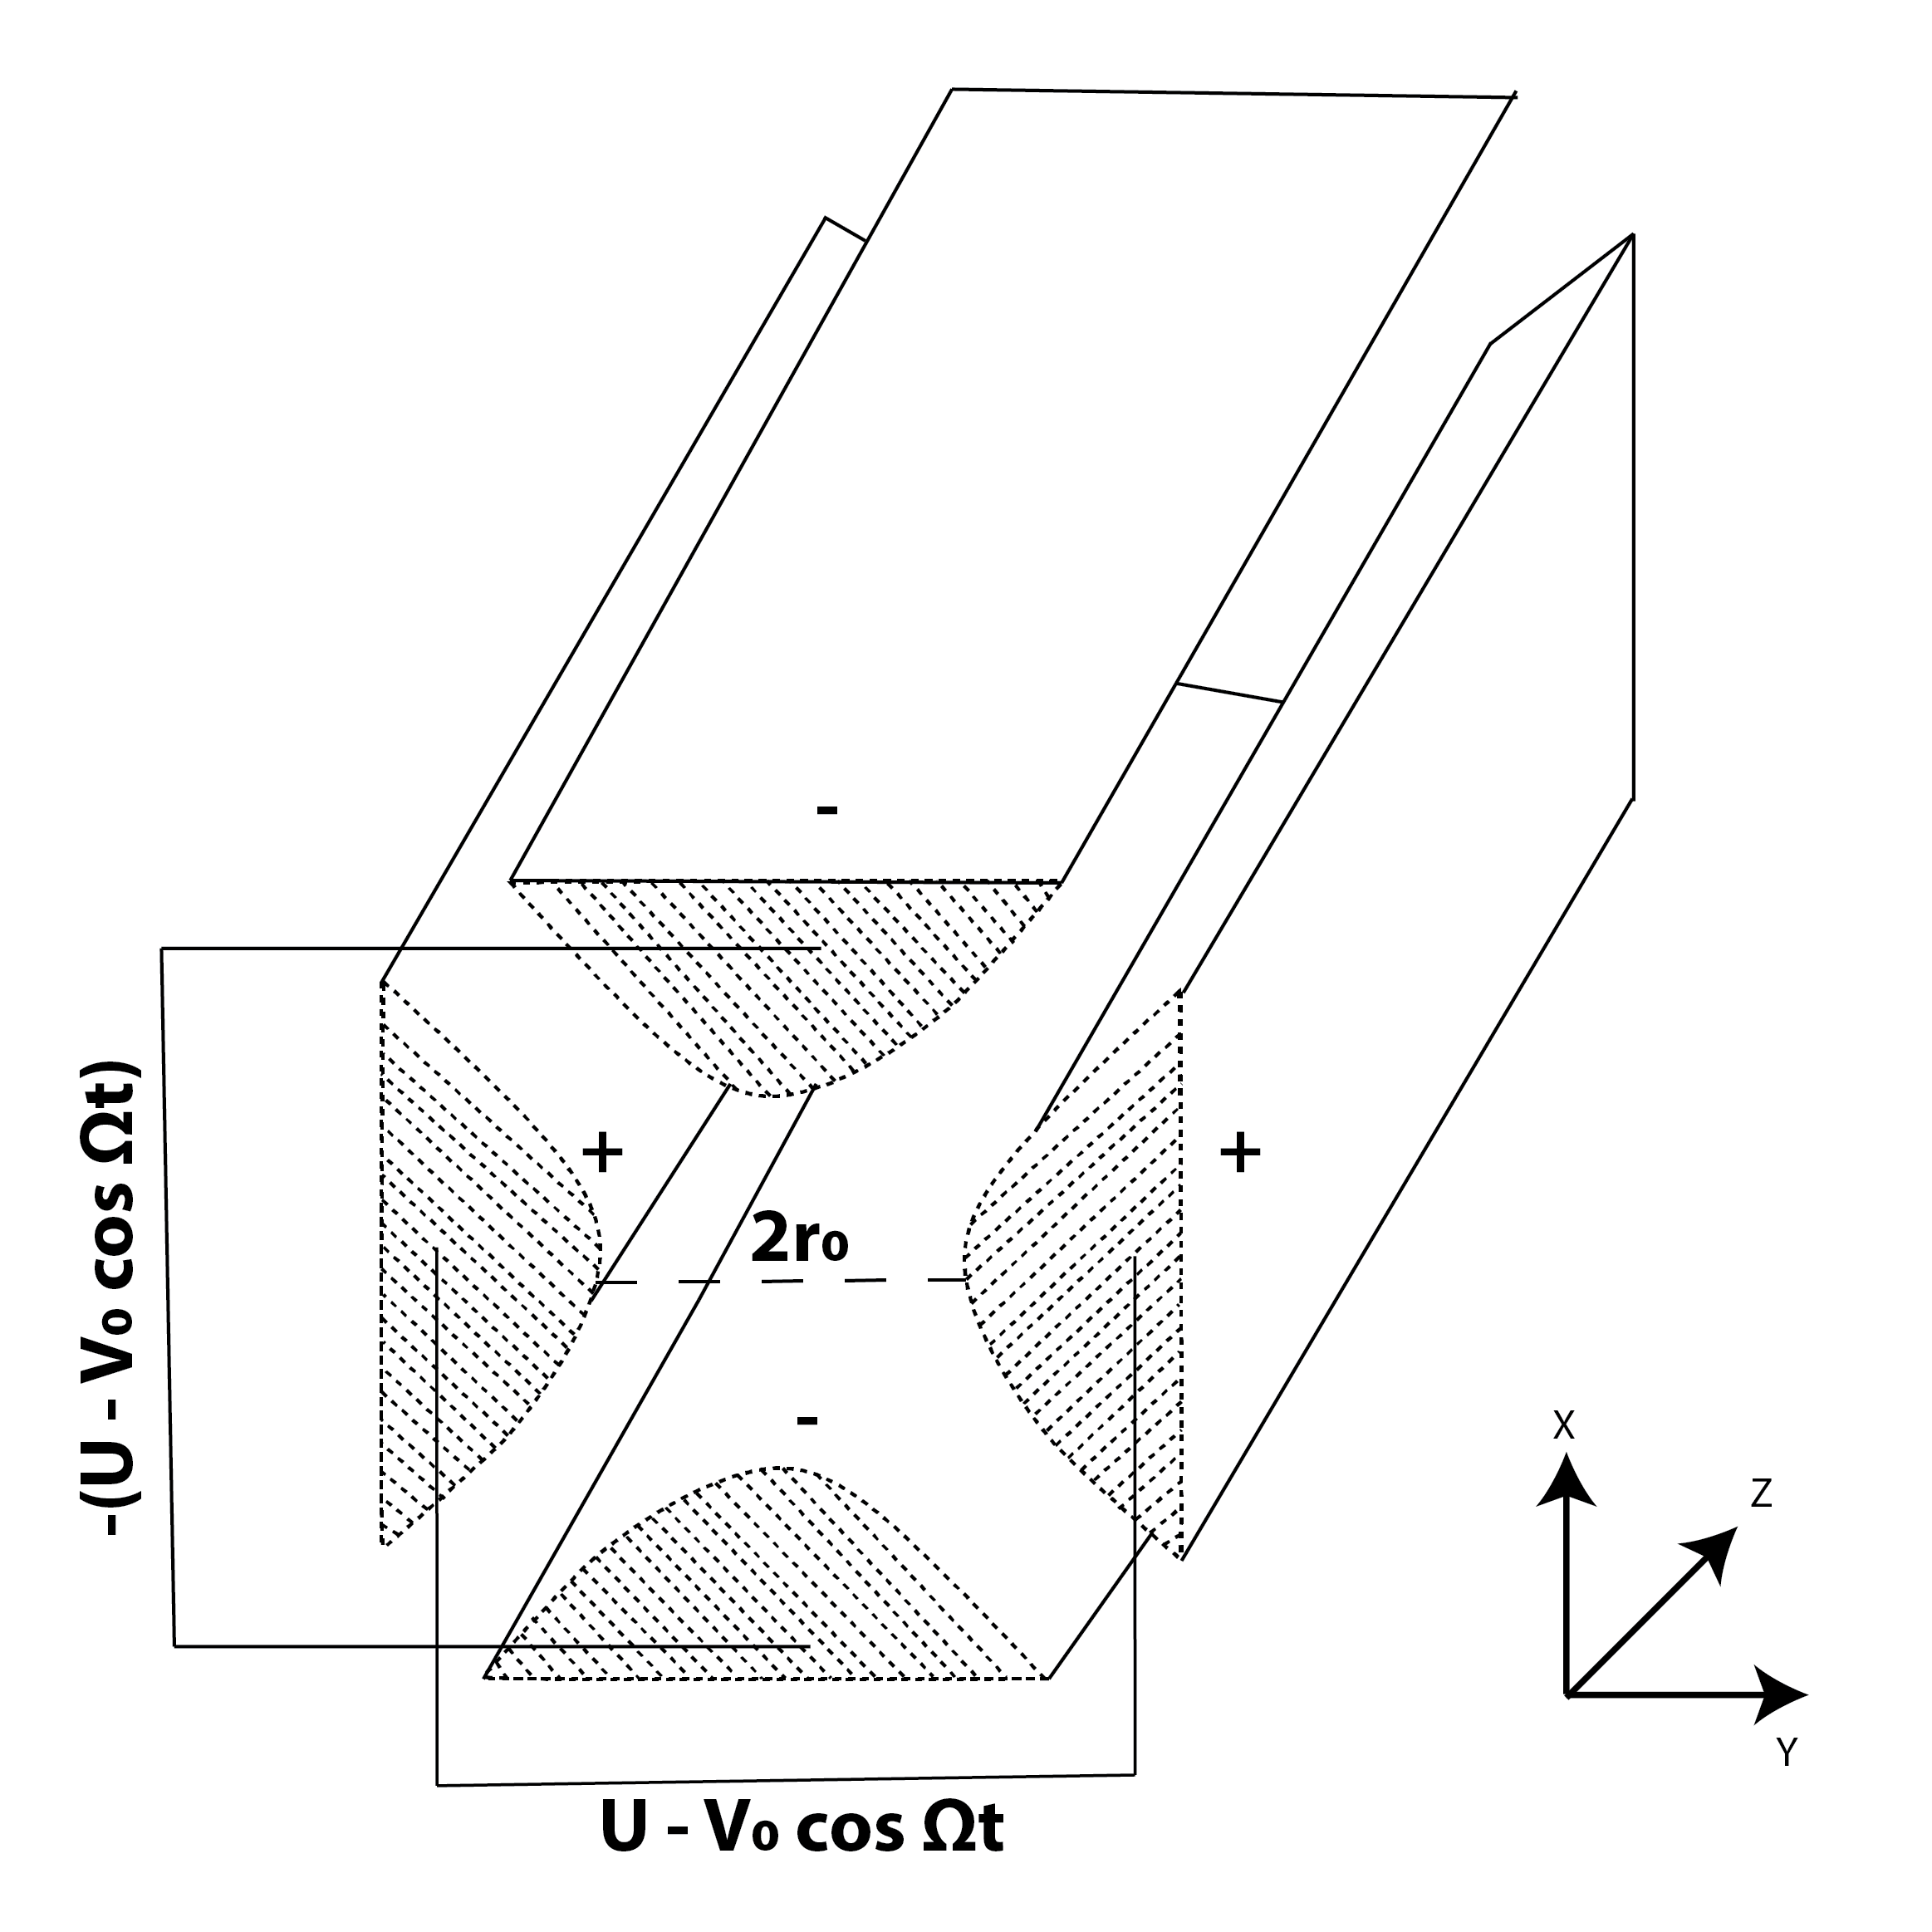
\includegraphics[width=0.5\textwidth]{figures/intro/trap/Quadrupole.png}
    \caption{Schematic diagram of a quadrupole mass filter. Ions enter and move along the z-axis as they oscillate in the x-y plane. The oscillation is regulated by applying DC (U) and radio frequency (RF) (V) potentials to each set of rods. Only ions with stable paths at the chosen U and V values will pass through the quadrupole mass filter.}
    \label{fig:quadrupole}
\end{figure}

\citet{paul_ionenka_1955} had developed the most basic electric field geometry known as the Paul or quadrupole ion trap. He also developed the quadrupole mass filter technique \cite{paul_elektrische_1955} (see Figure \ref{fig:quadrupole}). Using the combination of mass filter and ion trap, one can isolate and trap desired molecular ions with a specific mass-over-charge ratio ($m/z$). As a result, molecular spectroscopy in ions trap is routinely employed using action spectroscopic techniques \cite{SA2019, Roithovareview, Asvany2021}, as discussed in more detail in Section \ref{sec:action-spectroscopy}.

The trapped ions are usually cryogenically cooled to allow low temperatures experiments. Ion spectroscopic techniques typically employ collisional cooling with neutral buffer gas \cite{dehmelt_radiofrequency_1968, wester_radiofrequency_2009}. In the next section, we shall discuss the advantage of using a higher-multipole order ion trap, the 22-pole ion trap developed by \citet{gerlich_ion-neutral_1995}, and further improved by Asvany and Schlemmer \cite{asvany_note_2010} for low-temperature experiments under interstellar conditions.

\subsection{22-pole cryogenic ion trap}
\label{subsec:22-pole}

As discussed in Section \ref{subsec:intro:optical}, since the 1950s, ion chemistry under interstellar medium conditions has gained interest in exploring ion-molecule reactions at low temperatures and low-density \cite{smith_ion_1992, gerlich_experimental_1992}. Cryogenic ion trap experiments are commonly used to investigate laboratory ion-molecule reactions relevant to astrochemistry, and many astronomical objects have temperatures as low as 6 K \cite{harju_detection_2008}. However, in quadrupole traps, it is difficult to achieve low temperatures (kinetic and internal ion temperature) below $<10$ K \cite{gerlich_inhomogeneous_1992}. Therefore, higher-order multipole traps with large field-free zones are required for low-temperature astrochemical experiments.\\

\begin{figure}
    \centering
    \Subfigure[0.45]{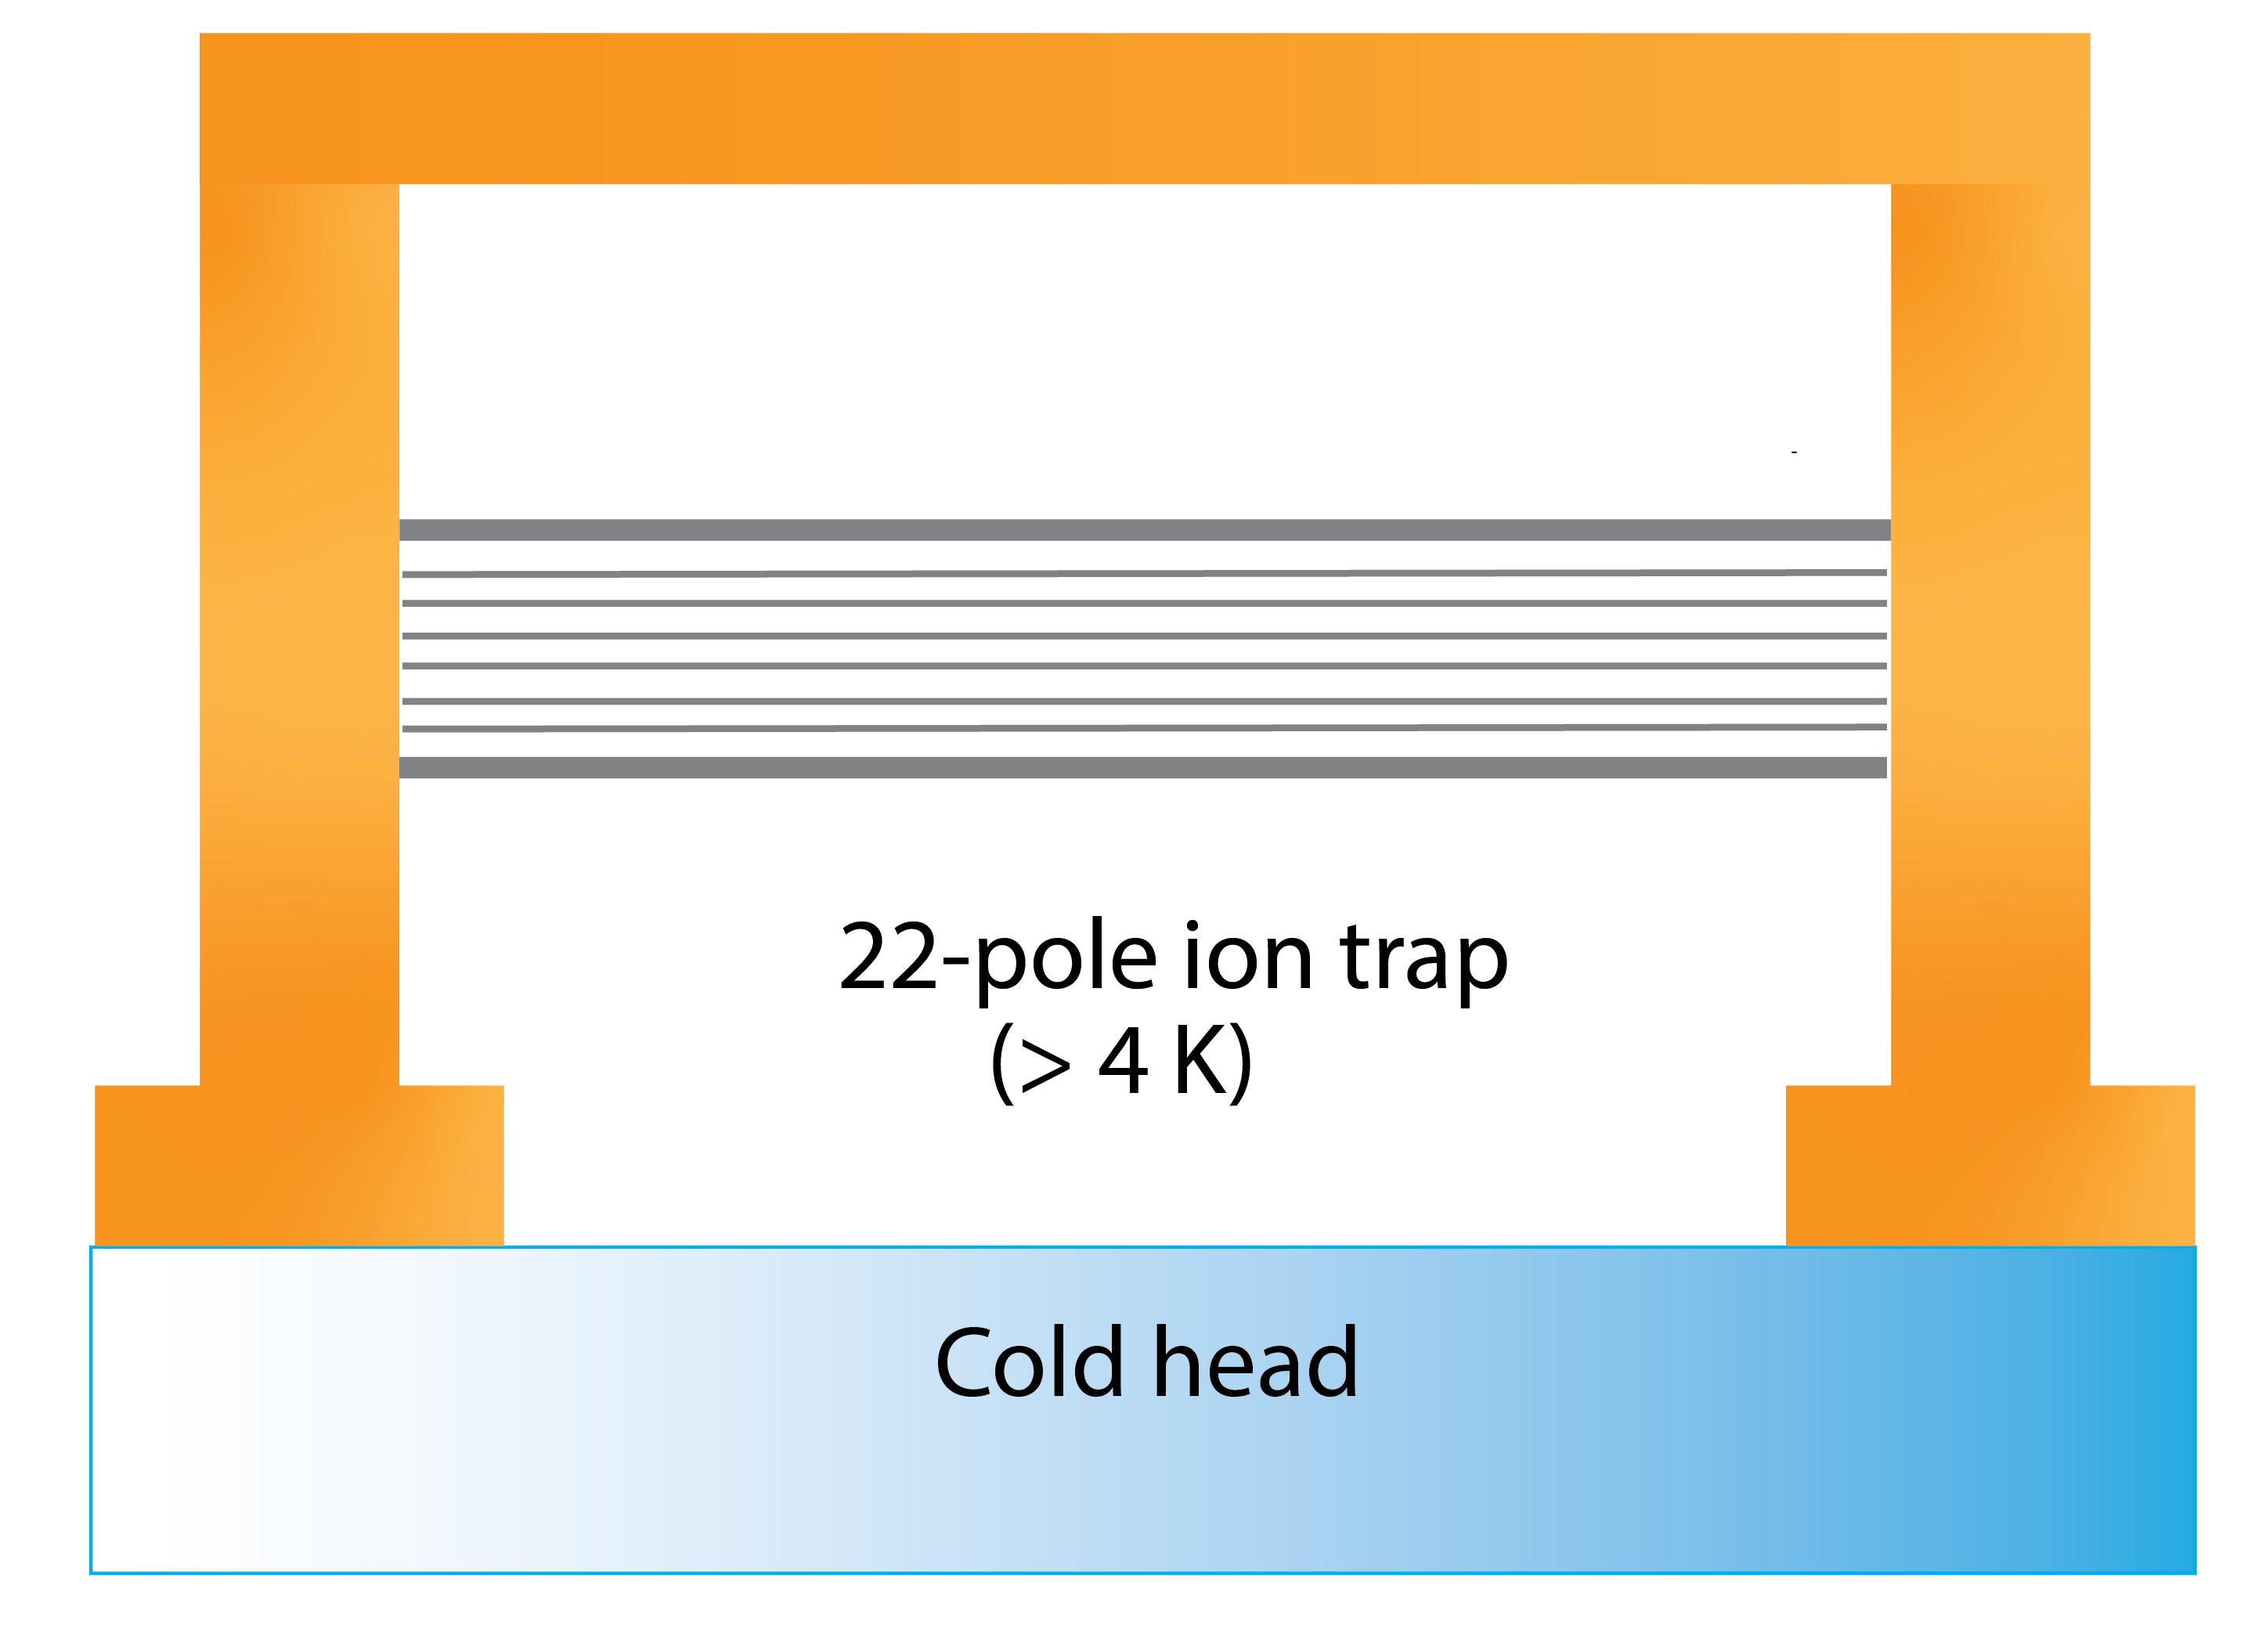
\includegraphics[width=1\textwidth]{figures/intro/trap/22-pole_ion - trap - coldhead.png}}{}{\label{fig:22-pole-iontrap-coldhead}}
    \hfill
    \Subfigure[0.5]{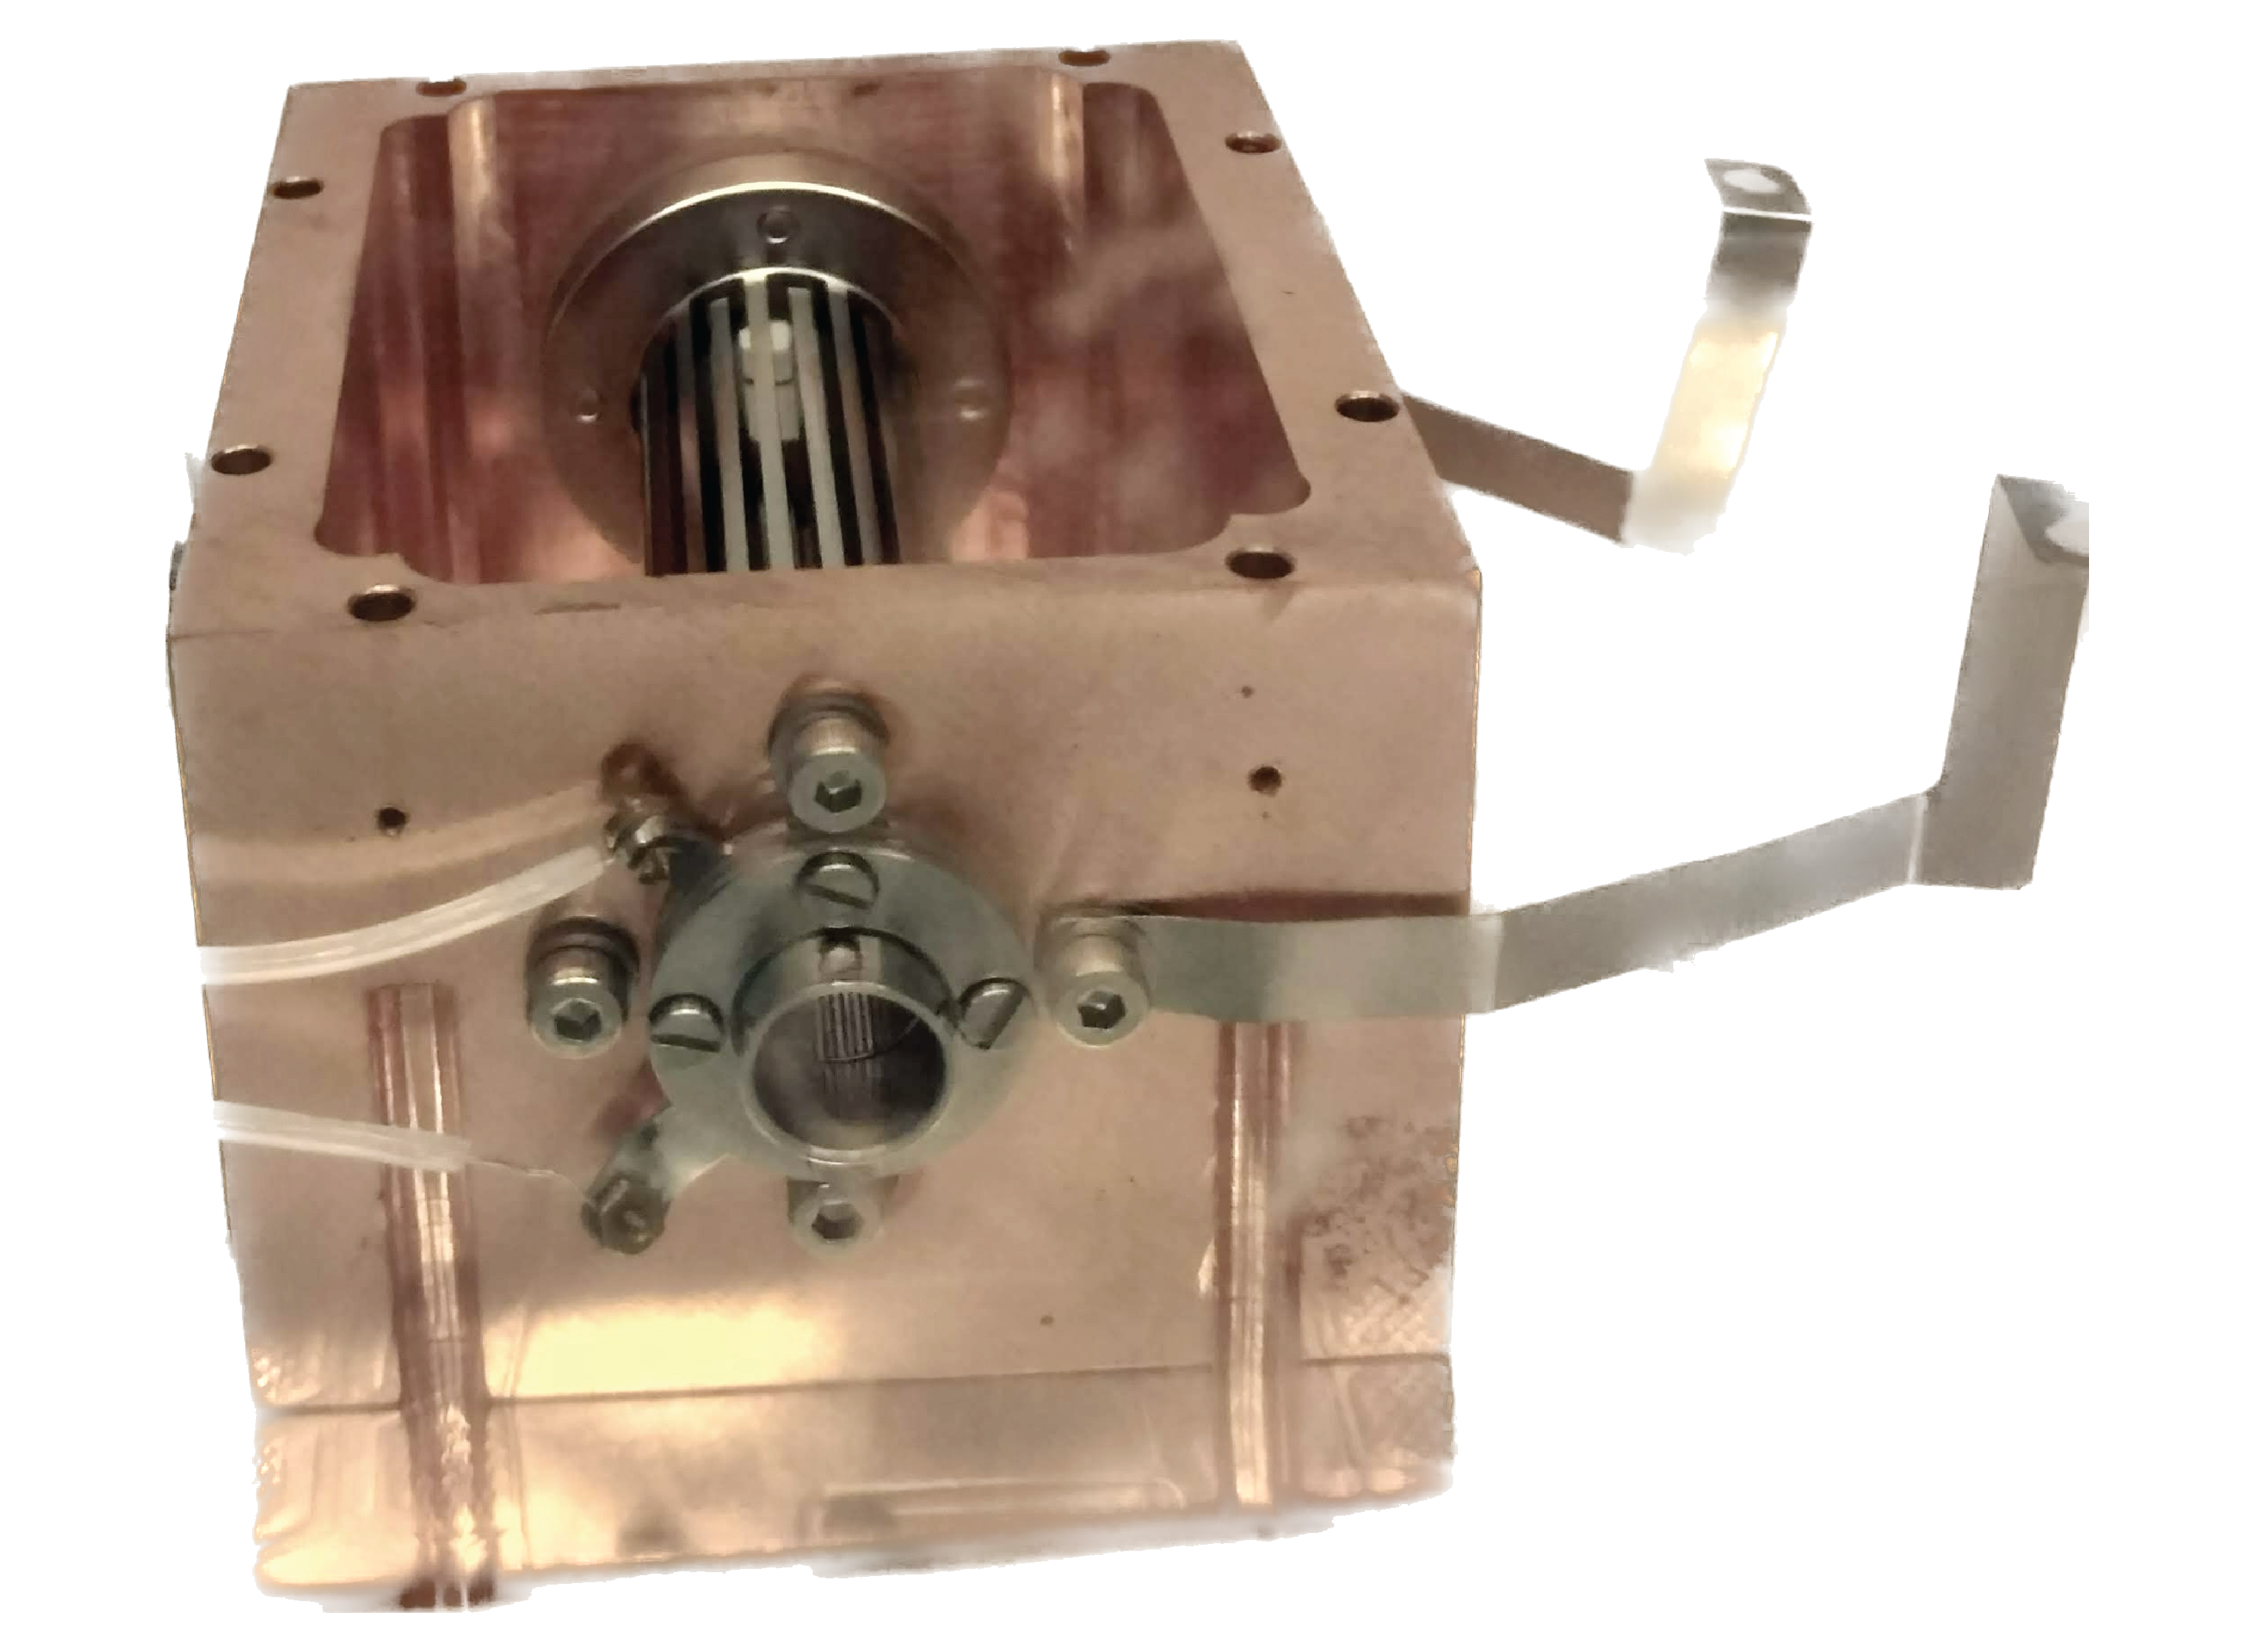
\includegraphics[width=1\textwidth]{figures/intro/trap/22PT.png}}{}{\label{fig:22PT-image}}
    
    \caption{(a) Schematic drawing of the 22-pole cryogenic ion trap (grey) in copper housing (orange) mounted onto cryogenic coldhead. (b) A photograph of the 22-pole ion trap mounted inside copper housing.}
    \label{fig:22PT}
\end{figure}

In a seminal review by \citet{gerlich_inhomogeneous_1992} titled \emph{Inhomogeneous rf fields: a versatile tool for the study of processes with slow ions}, the ideas of ion guiding and trapping using multipole fields have been described in great detail. Most notably, \citet{gerlich_ion-neutral_1995} also pioneered the development of the 22-pole ion trap (see Figure \ref{fig:22-pole-iontrap-coldhead}) for studies of ion-molecular reactions. The sensitivity and efficiency at low density and low temperature in 22-pole ion trap experiments is a major advantage over ion-molecule reaction studies at 300 K using other well-established techniques such as flowing afterglow (FA) \cite{fehsenfeld_thermalenergy_1967}, ion cyclotron resonance (ICR) ion traps \cite{kim_icr_1975}, and selected ion flow tube experiments (SIFT) \cite{smith_laboratory_1978}. With the development of the cryogenic 22-pole ion traps, significant advancements have occurred in studying low-temperature processes such as radiative association and three-body collisional processes in molecular complex formation \cite{gerlich_experimental_1992, paul_dynamics_1995, paul_deuteration_1996}.

The 22-pole cryogenic ion trap is also employed for high-resolution molecular spectroscopy of electronic \cite{chakrabarty_novel_2013, campbell_laboratory_2015}, vibrational \cite{asvany_understanding_2005} and rotational \cite{Brunken2017} transitions (see Section \ref{subsec:action:methods:vibrational} and \ref{subsec:action:methods:rotational}), including the first laboratory confirmation  of C$_{60}^+$ as the carrier of two DIBs by \citet{campbell_laboratory_2015}, using a 22-pole ion trap. It has gained even more popularity during the past two decades as a tool for researching ion-molecule interactions, and molecular ion spectroscopy  \cite{redwine_novel_2013, asvany_coltrap_2014, gunther_berlintrap_2017, jusko_felion_2019, rap_low-temperature_2022}.\\

In the next section, the action spectroscopic techniques developed in cryogenic ion traps for high-resolution molecular ion spectroscopy will be discussed.
